\section{Ejercicio 4}
\subsection{El Problema}
Dado un natural $L$, una matriz $M$, y un arreglo $ARR$ de $n$ matrices, el problema consiste en ver si existe un subarreglo de $ARR$ de tamaño $L$ cuyo producto sea $M$. En otras palabras, queremos ver si: 

\begin{center}
$(\exists   0 \leq i, j < n) (j - i = L - 1) \land (\displaystyle \prod_{i \leq k \leq j}^{} ARR_{k}) = M$
\end{center}

Como requerimiento del problema, nuestra solución tiene que cumplir con la cota de $O(n * log (n))$.
Por suerte, el enunciado nos garantiza que todas las matrices son de 3x3. Esto nos permitirá, por ejemplo, multiplicar 2 matrices en $O(1)$.
\subsection{Desarrollo}
Nuestra solución se divide principalmente en 3 partes. Para explicarlas, usaremos el siguiente ejemplo:
\begin{itemize}
\item $ARR = [A, B, C, D, E, F]$
\item $M = [BCD]$
\item $L = 3$
\end{itemize}
\subsubsection{Divide}
Comenzamos dividiendo nuestro arreglo de matrices a la mitad, y trabajamos con cada una por separado. Luego, repetimos el proceso con cada mitad, hasta que nuestras mitades tengan un tamaño menor o igual a $L$. Volviendo a nuestro ejemplo, se vería así:
\begin{figure}[H]
\centering
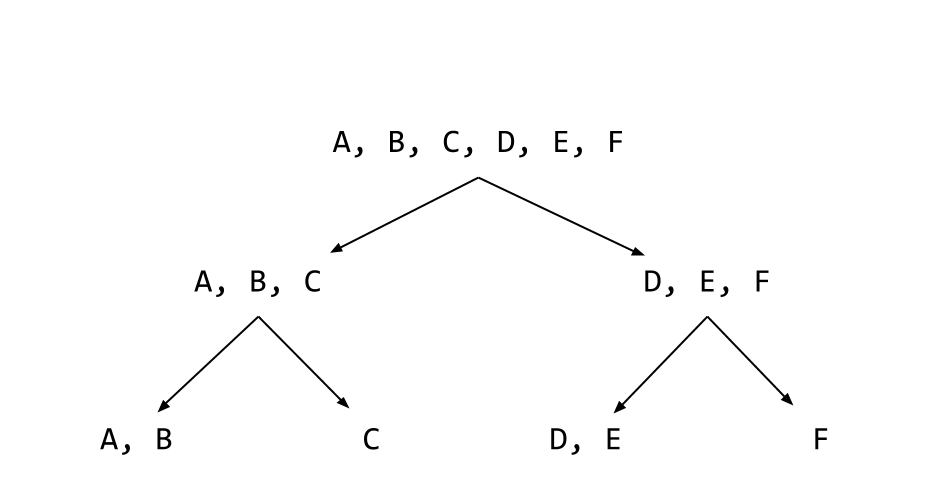
\includegraphics[scale=0.35]{Imagenes/ej4-ejem1}
\end{figure}
\subsubsection{Conquer}
Cada vez que dividimos nuestro arreglo, calculamos el producto de todas las matrices en el mismo. Cada producto realizado es almacenado. Si tuviesemos el arreglo $[X, Y, Z]$, el producto almacenado sería $[X, XY, XYZ]$. Una vez más, viendo nuestro ejemplo, sería así:
\begin{figure}[H]
\centering
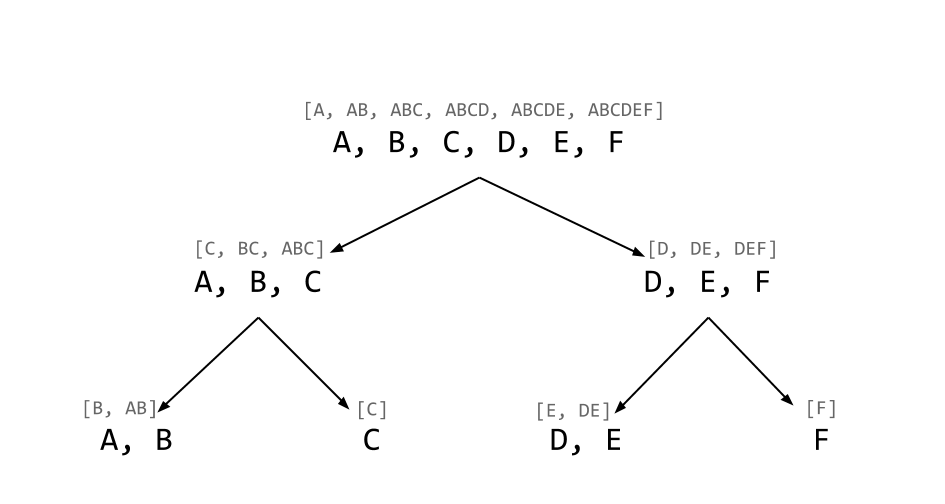
\includegraphics[scale=0.35]{Imagenes/ej4-ejem2}
\end{figure}

En esta imagen podemos ver dos cosas. Primero, que se calculan de forma diferente los productos de la mitades izquierdas, que el de las derechas. Esto se debe a que al calcular este producto, comenzamos desde lo que sería el centro hacia afuera (la razón se explica en el siguiente punto). Segundo, si un subarreglo tiene tamaño $L$, inmediatemente nos podemos fijar si el producto final es igual a $M$ o no. Si lo fuese, ya podemos decir que existe el subarreglo buscado y terminar la ejecución. 

Cabe destacar que si bien el producto de $[A, B, C, D, E, F]$ es en efecto [$A$, $AB$, $ABC$, $ABCD$, $ABCDE$, $ABCDEF$], no tiene sentido calcular un producto de más de $L$ matrices. Por lo tanto, en la práctica, solo calcularemos $[A, AB, ABC]$ . En entonces que está parte del algoritmo tiene complejidad $O(L)$, ya que recorremos el arreglo linealmente, multiplicando siempre 2 matrices entre ellas, y como mucho lo haremos $L$ veces.

\subsubsection{Combine}
Ya dijimos que si uno de los subarreglos armados tiene como producto a $M$, terminamos. El problema es que nuestro $M$ del ejemplo no es ninguna de las mitades obtenidas, pero igualmente existe dentro de $ARR$. Lo que tenemos que hacer entonces es encontrar este subarreglo al momento de unir las dos mitades. Es por eso que si una mitad no produce a $M$, entonces devuelve su producto para poder ser combinado.

\begin{figure}[H]
\centering
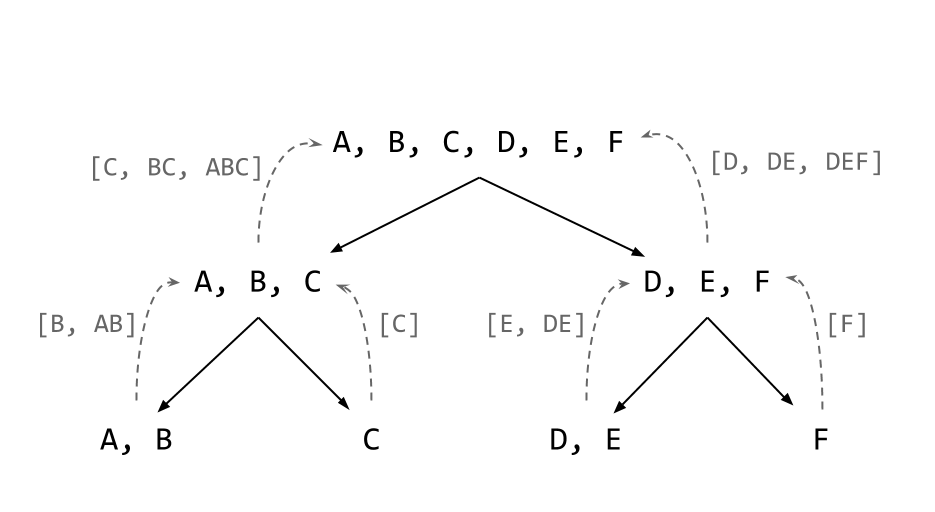
\includegraphics[scale=0.35]{Imagenes/ej4-ejem3}
\end{figure}

Veamos este caso en particular:

\begin{figure}[H]
\centering
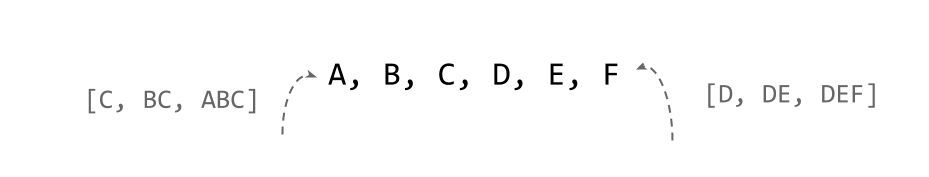
\includegraphics[scale=0.35]{Imagenes/ej4-ejem4}
\end{figure}

Vamos a querer unir esta información para ver si existe el subarreglo buscado.

\begin{figure}[H]
\centering
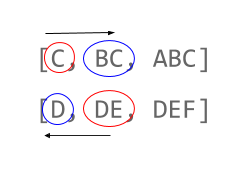
\includegraphics[scale=0.7]{Imagenes/ej4-ejem5}
\end{figure}

En este caso en particular, tenemos que unir $C$ con $DE$, y $BC$ con $D$. En cada uno de estos productos, comparamos con $M$ para ver si encontramos el subarreglo deseado. No es casualidad que los arreglos de productos tengan la forma que tienen. Los construimos de esta forma para poder avanzar en uno mientras retrocedemos en otro al ir calculando los productos. 

Es por eso que unir esta información tiene complejidad $O(L)$, ya que nuevamente estamos recorriendo linealmente los arreglos (de tamaño máximo $L$), y haciendo una multiplicación de 2 matrices en cada paso.

Finalmente, logramos calcular todos los productos de subarreglos posibles. Si encontramos un producto igual a $M$, terminamos la ejecución imprimiendo un "SI". Si no lo encontramos, imprimiremos un "NO".
\subsubsection{Complejidad}
Dado que siempre estamos dividiendo el arreglo a la mitad, tenemos $log(n)$ llamadas recursivas. Y en cada paso, el $Conquer$ y el $Combine$ tienen complejidad $O(L)$. Por lo tanto, la complejidad final del algoritmo es $O(L * log(n))$. Ahora, como $L \leq n$, terminamos con $O(n * log(n))$

Más formalmente, podemos aplicar el teorema maestro donde:

$T(n)=2T\left({\frac {n}{2}}\right)+O(n)$	 (al igual que $Merge Sort$).

Por lo tanto, la complejidad termina siendo $O(n * log(n))$.

Si bien la implementación coíncide con la descripción planteada, cabe aclarar que al momento de calcular el producto de las matrices utilizamos la operación de $push\_back$ \textsuperscript{\cite{pushback}} de $vector$. La misma tiene un costo $O(1)$ amortizado, por lo que la consideraremos $O(1)$ en nuestros cálculos de complejidad.